\documentclass[13pt]{article}

\usepackage[T1]{fontenc}
\usepackage[utf8]{inputenc}

\usepackage[hidelinks]{hyperref}

\usepackage{microtype}

\usepackage{amssymb}
\usepackage{amsmath}
\usepackage{mathtools}
\usepackage{dsfont}

\usepackage{enumitem}

\usepackage{tikz}
\usetikzlibrary{cd, patterns, patterns.meta, decorations.pathmorphing}

\usepackage{geometry}
\geometry{a4paper, total={170mm, 252mm}, top=22mm}

\usepackage[skip=7pt]{parskip}

\usepackage{amsthm}
\usepackage{thmtools}

\declaretheoremstyle[
    headfont=\bfseries\color{green!80!black},
    bodyfont=\normalfont,
    notebraces={: }{},
    notefont=\color{green},
    headformat=\NAME$\;$\NUMBER\NOTE,
    postheadspace=\newline,
    mdframed={
        linewidth=2pt,
        rightline=false, topline=false, bottomline=false,
        linecolor=green, backgroundcolor=yellow!4,
        skipabove=3mm, skipbelow=3mm
    }
]{defbox}

\declaretheoremstyle[
    headfont=\bfseries\color{orange!80!black},
    bodyfont=\normalfont,
    notebraces={: }{},
    notefont=\color{orange},
    headformat=\NAME$\;$\NUMBER\NOTE,
    postheadspace=\newline,
    mdframed={
        linewidth=2pt,
        rightline=false, topline=false, bottomline=false,
        linecolor=orange, backgroundcolor=yellow!4,
        skipabove=3mm, skipbelow=3mm
    }
]{theorembox}

\declaretheoremstyle[
    headfont=\bfseries\color{blue!80!black},
    bodyfont=\normalfont,
    notebraces={: }{},
    notefont=\color{purple},
    headformat=\NAME$\;$\NUMBER\NOTE,
    postheadspace=\newline,
    mdframed={
        linewidth=2pt,
        rightline=false, topline=false, bottomline=false,
        linecolor=purple, backgroundcolor=yellow!4,
        skipabove=3mm, skipbelow=3mm
    }
]{lemmabox}

\declaretheoremstyle[
    headfont=\bfseries\color{orange!80!black},
    bodyfont=\normalfont,
    notebraces={: }{},
    notefont=\color{orange},
    headformat=\NAME$\;$\NUMBER\NOTE,
    postheadspace=\newline,
    mdframed={
        linewidth=2pt,
        rightline=false, topline=false, bottomline=false,
        linecolor=red!50!orange, backgroundcolor=yellow!4,
        skipabove=3mm, skipbelow=3mm
    }
]{conclusionbox}

\newtheoremstyle{straightstyle}
  {6pt} % Space above
  {6pt} % Space below
  {} % Body font
  {} % Indent amount
  {\bfseries} % Theorem head font
  {.} % Punctuation after theorem head
  {.5em} % Space after theorem head
  {} % Theorem head spec (can be left empty, meaning `normal')

\newtheoremstyle{italicsstyle}
  {6pt} % Space above
  {6pt} % Space below
  {\slshape} % Body font
  {} % Indent amount
  {\bfseries} % Theorem head font
  {.} % Punctuation after theorem head
  {.5em} % Space after theorem head
  {} % Theorem head spec (can be left empty, meaning `normal')

\declaretheorem[ %
  name=Definition, %
  numberwithin=section, %
  style=defbox
]{definition}

\declaretheorem[ %
  name=Theorem, %
  numberwithin=section, %
  style=theorembox
]{theorem}

\declaretheorem[ %
  name=Proposition, %
  numberlike=theorem, %
  style=theorembox
]{proposition}

\declaretheorem[ %
  name=Corollary, %
  numberlike=theorem, %
  style=straightstyle
]{corollary}

\declaretheorem[ %
  name=Lemma, %
  numberlike=theorem, %
  style=lemmabox
]{lemma}

\declaretheorem[ %
  name=Remark, %
  numberlike=definition, %
  style=italicsstyle
]{remark}



\declaretheorem[ %
  name=Conclusion, %
  numberlike=theorem, %
  style=conclusionbox
]{conclusion}

\declaretheorem[ %
  name=Example, %
  numberwithin=section, %
  style=straightstyle
]{example}



% \renewenvironment{proof}{{\bfseries Proof}$ $\newline}{
%   \begin{flushright} $ \spadesuit $ \end{flushright}$ $\newline
% }

\usepackage{cleveref}

%\crefname{definition}{definicja}{definicje}
%\Crefname{definition}{Definicja}{Definicje}
%
%\crefname{theorem}{twierdzenie}{twierdzenia}
%\Crefname{theorem}{Twierdzenie}{Twierdzenia}
%
%\crefname{lemma}{lemat}{lematy}
%\Crefname{lemma}{Lemat}{Lematy}
%
%\crefname{remark}{uwaga}{uwagi}
%\Crefname{remark}{Uwaga}{Uwagi}


\DeclareMathOperator{\Z}{\mathbb{Z}}
\DeclareMathOperator{\R}{\mathbb{R}}
\DeclareMathOperator{\C}{\mathbb{C}}
\DeclareMathOperator{\N}{\mathbb{N}}
\DeclareMathOperator{\Q}{\mathbb{Q}}

\DeclareMathOperator{\im}{im}
\DeclareMathOperator{\coker}{coker}

\newcommand{\set}[1]{\mathcal{#1}}


\DeclareMathOperator{\ord}{ord}
\DeclareMathOperator{\Ann}{Ann}
\DeclareMathOperator{\Hom}{Hom}

\DeclareMathOperator{\End}{End}

\let\landtemp\land
\renewcommand{\land}{\;\landtemp\;}





\usepackage{tikz}
\usetikzlibrary{spath3, hobby, knots, braids}

\pgfdeclarelayer{bg}    % declare background layer
\pgfsetlayers{bg,main}

\title{A voyage into the algebras}
\author{
  Weronika Jakimowicz\\
  330006
  \and 
  Julia Walczuk\\
  332742
}
\date{2023-2024}

\begin{document}
\maketitle
\bigskip

%\begin{center}
%  \begin{tikzpicture}
%    \begin{knot}[
%      consider self intersections,
%      flip crossing=2,
%      clip width=10,
%      ]
%      \strand[thick]
%      (90:2) to[out=180,in=-120,looseness=2]
%      (-30:2) to[out=60,in=120,looseness=2]
%      (210:2) to[out=-60,in=0,looseness=2] (90:2);
%    \end{knot}
%
%  \fill (0,0) circle (2pt);
%\fill(90:2) circle (2pt);
%\fill(-30:2) circle (2pt);
%\fill(210:2) circle (2pt);
%  \end{tikzpicture}
%\end{center}
%
%\begin{center}
%  \begin{tikzpicture}
%    \begin{knot}[
%      consider self intersections,
%      flip crossing=2,
%      clip width=10,
%      ]
%      \strand[thick]
%      (120:2) to[out=180, in=180, looseness=2] (210:1) to[out=0, in=-140, looseness=1] (40:0.6) to[out=40, in=180, looseness=0.5] (40:1) to[out=5, in=-5, looseness=3] (-40:1) to[out=180, in=0, looseness=0.5] (150:1) to[out=180, in=180, looseness=2] (-120:2) to[out=0, in=0, looseness=1.3] (120:2);
%    \end{knot}
%%\fill (120:2) circle (2pt);
%%\fill (-120:2) circle (2pt);
%%\fill (-40:1) circle (2pt);
%%\fill (40:1) circle (2pt);
%%\fill (150:1) circle (2pt);
%%\fill (210:1) circle (2pt);
%%\fill[green] (40:0.6) circle (2pt);
%%\fill[red] (0,0) circle (2pt);
%  \end{tikzpicture}
%\end{center}
\newpage

%\section{Problem}

{\bfseries%
  Consider the ring $\Z[[F]$, where $[F]$ is the equivalence class of all finite abelian groups isomorphic to $F$. Describe the set $\Z[[F]]/\{[F_2]=[F_1]+[F_3]\}$, where relation $[F_2]=[F_1]+[F_3]$ means that there exists exact sequence:

  \begin{center}\begin{tikzcd}
    0\arrow[r] & F_1\arrow[r] & F_2\arrow[r] & F_3\arrow[r] & 0
  \end{tikzcd}\end{center}
}

Every finite abelian group is isomorphic to either a cyclic group or a finite product of cyclic groups. We will use this fact alongside the knowledge that every cyclic group is isomorphic with $\Z_n$ for some $n\in\N$.

We will start by showing that if $n=k\cdot l$ then $[\Z_n]=[\Z_k]+[\Z_l]$. Consider the sequence

\begin{center}\begin{tikzcd}
  0 \arrow[r] & \Z_k \arrow[r, "f"] & \Z_{n} \arrow[r, "g"] & \Z_l \arrow[r] & 0
\end{tikzcd}\end{center}

Define $f(1)=l\mod n$ and $g(1)=1\mod l$. We now need to check if $\ker g=\im f$. Take any $x\in\ker g$, then $x=l\cdot m\mod n$ for some $m\in\{0, 1, 2, ..., k-1\}$. Then for $m\mod l\in\Z_l$ we have $f(m\mod l)=ml\mod n$ and so $x\in\ker g\iff x\in \im f$. This shows that the sequence above is exact and $[\Z_n]=[\Z_k]+[\Z_l]$.

Furthermore, if $n=\prod_{i\leq m}k_i$, then
$$[\Z_n]=[\Z_{\prod_{i\leq m-1}k_i}]+[\Z_{k_m}]=...=\sum_{i\leq m}[\Z_{k_i}]$$
and if $n=p^k$ then by applying the above equation we have $[\Z_n]=k[\Z_p]$.

Next, we observe that for any $n,k\in\Z$ $[\Z_n\oplus \Z_k]=[\Z_n]+[\Z_k]$. This is because

\begin{center}\begin{tikzcd}
  0\arrow[r] & \Z_n \arrow[r, "f"] & \Z_n\oplus \Z_k \arrow[r, "g"] & \Z_k \arrow[r] & 0
\end{tikzcd}\end{center}

with $f(x)=x\oplus 0$ and $g(x\oplus y)=y$ is an exact sequence. For any $x\oplus y\in\ker g$ we must have $y=0$ while $x$ is unrestricted thus $x\oplus y\in \im f$.

From the latter statement, the following equality is immediately obtained:
\begin{align*}
  \Bigl[\bigoplus_{i\leq n}\Z_{k_i}\Bigr]=\Bigl[\bigl(\bigoplus_{i\leq n-1} \Z_{k_i}\bigr)\oplus \Z_{k_n}\Bigr]=\Bigl[\bigoplus_{i\leq n-1}\Z_{k_i}\Bigr]+[\Z_{k_n}]=...=\sum_{i\leq n}[\Z_{k_i}]
\end{align*}

If $F_n$ and $F_n'$ are two abelian groups of order $n$ and if $F_n=\bigoplus_{i\leq m}\Z_{k_i}$ then we have
$$[F_n]=\sum_{i\leq m} [\Z_{k_i}]$$
But because $n=|F_n|=|\oplus \Z_{k_i}|=\prod k_i$, then from the first two observations we obtain
$$[F_n']=\sum_{i\leq m} [\Z_{k_i}]$$
and so $[F_n]=[F_n']$. This allows us to replace every $\sum n_i[F_i]\in\Z[[F]$ with $\sum k_i[\Z_{p_i}]$ for prime $p_i$. Therefore,
$$\Z[[F]/\{[F_2]=[F_1]+[F_3]\}=\{\sum_{i\leq n} k_i[\Z_{p_i}]\;:\;p_i\text{ are prime}, n,k_i\in\N\}$$


\section{Introduction}

\subsection{Order of an Ideal over PID ring}

PID -> every ideal is generated by one element, every module is an image of a free module, hence it can be expressed as $M\cong R/I_1\oplus...\oplus R/I_n$ for some ideals $I_i$. This allows as to define order of a module as $\ord(M)=\ord(I_1...I_n)$, which is the element that generates the ideal $I_1....I_n$. 

$\ord(M)$ can also be described using equivalence relation $M\sim M_1 + M_2\iff 0\to M_1\to M\to M_2\to 0$ is an exact sequence -> finitely generated abelian groups as $\Z$ modules and vector fields over $\mathfrak{K}$ as $\mathfrak{K}[x]$-modules.

\subsection{The Problem of non-PID rings}

Not every ring is a PID -> we must either find another invariant or make the ring in question a PID. E.g. for $\Z[x, x^{-1}]$ we can tensor it with some field, usually $\Q$ but we might want to try $F_p$ for some prime $p$.

Maybe some example for $\Z[x]$?

\subsection{Short Introduction to Knot Theory?}

Knot - a closed curve immersed in some $3$-dimensional space, or $S^1$ immersed in $S^3$

We will consider only tamed knots? That is knots that can be represented as a sum of a finite amount of straight lines?

Using Mayer-Vietoris sequence we can deduce that $H^1(S^3\setminus K)=\Z$ for any knot $K$. Hence, if we want to find interesting invariants, we must look further. 

Seifert surface of knot $K$ is an orientable surface whose boundary is $K$. We can use it to create an infinite cyclic covering of $S^3\setminus K$ by cutting copies $S^3\setminus K$ along this surface and gluing the $+$ side of Seifert surface of one copy to the $-$ side of the next copy.

$H^1(K^*)$ is more complicated than $H^1(S^3\setminus K)$ and things get interesting if we consider it as a $\Z[\Z]$ (or $\Z[x, x^{-1}]$-module. We can use the fact that $\Pi_1(K^*)^{ab}=H^1(K^*)$ and calculate this module to obtain something called Alexander ideal $I$: $H^1(K^*)\cong \Z[\Z]/I$. If $I$ is a principal ideal, e.g. in the case of trefoil knot of figure eight knot, its generator is called "Alexander polynomial". If this is not the case, we must consider $H^1(K^*; \Q)$ - kohomology module with coefficients in $\Q$, to obtain the Alexander polynomial. In the following paper we will consider what happens if we use $F_p$, a finite field, instead of $\Q$.


%\section{Calculating the Alexander Module}

Kinoshita-Tarasaki - does not look too promising

Conway Knot - to be examined


\section{The case of oriented knot diagrams}

\subsection{Labeling homomorphism with orientation}

Every knot diagram can be endowed with orientation in two different ways. Given an oriented knot diagram there are two distinct types of crossings as seen in \cref{fig:4:two:types:crossings}. In such crossings segments $i$ and $o$ are easily distinguishable, allowing us to write two different elements to which labeling homomorphism $\phi$ will map segments that contribute to one crossing:
$$+:\phi(u,i,o)=au+bi+co$$
$$-:\phi(u,i,o)=\alpha u+\beta i+\gamma o.$$

\begin{figure}[h]\centering
  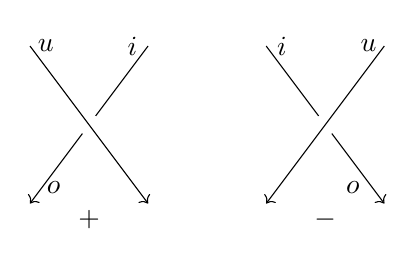
\begin{tikzpicture}
    \draw[<-] (0, -2)--(1.5, 0);
    \fill[white] (0.75, -1) circle (4pt);
    \draw[->] (0, 0)--(1.5, -2);

    \node at (0.75, -2.2) {$+$};
    \node at (0.2, 0) {$u$};
    \node at (1.3, 0) {$i$};
    \node at (0.3, -1.8) {$o$};

    \draw[->] (3, 0)--(4.5, -2);
    \fill[white] (3.75, -1) circle (4pt);
    \draw[<-] (3, -2)--(4.5, 0);
    
    \node at (3.75, -2.2) {$-$};
    \node at (3.2, 0) {$i$};
    \node at (4.3, 0) {$u$};
    \node at (4.1, -1.8) {$o$};
  \end{tikzpicture}
  \caption{\label{fig:4:two:types:crossings}Two types of crossings in oriented knot diagram.}
\end{figure}

Just as before, elements from $M^s$ that map to $0$ element in $M^x$ are responsible for coloring of the diagram being examined.

Those two definitions of homomorphism can be used to define two operators $M\times M\to M\times M$ which take segments that enter a crossing and return segments that leave said crossing. Looking from top to bottom of \cref{fig:4:two:types:crossings}, said operators are represented by matrices:
$$
A_+=\begin{pmatrix}
  -c^{-1}a & -c^{-1}b \\
  1 & 0
\end{pmatrix}
\begin{pmatrix}u\\i\end{pmatrix}
\quad\quad\quad
A_-=\begin{pmatrix}
  0 & 1 \\ 
  -\gamma^{-1}\beta & -\gamma^{-1}\alpha
\end{pmatrix}
\begin{pmatrix}i\\u\end{pmatrix}
$$


%\section{Problem}

Consider a field $\mathfrak{K}$ and the ring of polynomials with coefficients in $\mathfrak{K}$, $\mathfrak{K}[x]$. Obviously, the aforementioned ring is a principial ideal domain. We want to consider group $\Z[[M]]$, where $[M]$ is the equivalence class of all finitely generated torsion modules isomorphic to $M$ and relation $[M_2]=[M_1]+[M_3]$ defined by the existence of an exact sequence.

Any finitely generated module $M$ is isomorphic to a direct sum of cyclic modules:
$$M\cong p_1\mathfrak{K}[x]\oplus p_2\mathfrak{K}[x]\oplus...\oplus p_n\mathfrak{K}[x]$$

Moduły które mają ten sam wielomian w rozkładzie trafiają do tego samego domku.

{\color{green} If $p$, $q$ are two irreducible polynomials, then $(p)\oplus  (q)=\mathfrak{K}[x]$ (example: $x-1, x^2+1$).}


$$x^2+2x+1-(x-1)(x+3)$$


\bibliographystyle{plain}
\bibliography{literatura}
 
\end{document}
